\section{Clustering}


\begin{frame}{Clustering: Background}
    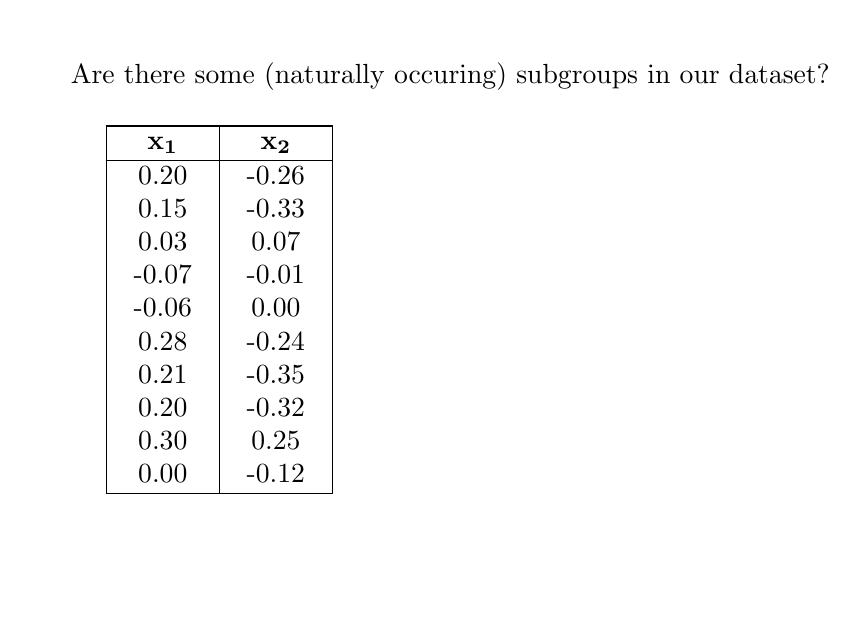
\begin{tikzpicture}
        \node[] at (-5.25, 3.5) {};
        \node[] at (-5.25, -3.5) {};

        \node[] at (0, 3) {
            Are there some (naturally occuring) subgroups in our dataset?
        };

        \visible<2>{
            \node[anchor=north west] at (-4.5, 2.5) {
                \begin{tabular}{|>{\centering\arraybackslash}p{1cm}|>{\centering\arraybackslash}p{1cm}|}
                    \hline
                    $\mathbf{x_1}$ & $\mathbf{x_2}$ \\
                    \hline
                    0.20&-0.26\\
                    0.15&-0.33\\
                    0.03&0.07\\
                    -0.07&-0.01\\
                    -0.06&0.00\\
                    0.28&-0.24\\
                    0.21&-0.35\\
                    0.20&-0.32\\
                    0.30&0.25\\
                    0.00&-0.12\\
                    \hline
                \end{tabular}
            };
        }
    \end{tikzpicture}
\end{frame}
